\documentclass[14 pt]{extarticle}

	\usepackage[frenchb]{babel}
	\usepackage[utf8]{inputenc}  
	\usepackage[T1]{fontenc}
	\usepackage{amssymb}
	\usepackage[mathscr]{euscript}
	\usepackage{stmaryrd}
	\usepackage{amsmath}
	\usepackage{tikz}
	\usepackage[all,cmtip]{xy}
	\usepackage{amsthm}
	\usepackage{varioref}
	\usepackage{geometry}
	\geometry{a4paper}
	\usepackage{lmodern}
	\usepackage{hyperref}
	\usepackage{array}
	 \usepackage{fancyhdr}
	 \usepackage{float}
\renewcommand{\theenumi}{\alph{enumi})}
	\pagestyle{fancy}
	\theoremstyle{plain}
	\fancyfoot[C]{} 
	\fancyhead[L]{Interrogation}
	\fancyhead[R]{9 mars 2022}\geometry{
 a4paper,
 total={170mm,257mm},
 left=20mm,
 top=20mm,
 }
	
	
	\title{Interrogation chapitre 6}
	\date{}
	\begin{document}

\begin{center}{\Large Interrogation chapitre 6}\\ 
 \end{center}
 Nom : \ldots\ldots\ldots\\
 Prénom : \ldots\ldots\ldots
 
 \subsection*{Exercice 1}
 Complétez directement sur l'énoncé : 
 
 \begin{enumerate}
 \item $\frac75 + \frac45 =  $ 
 \item $\frac58 - \frac78=  $ 
 \item $\frac17 + \frac14 =  $
 \item $\frac53 - \frac25 +  \frac1{15} =  $
 \end{enumerate}
 
\subsection*{Exercice 2} 
 
On considère la figure suivante, avec $MH = 18$, $MS= 12$, $SH = 9$, et $MA = 4,5$. 

 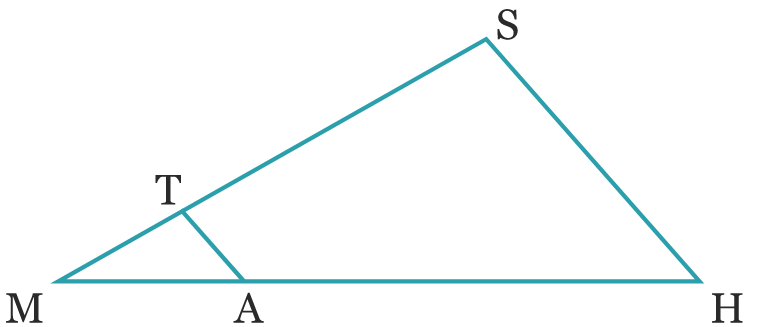
\includegraphics[scale=.3]{Exo3.png}\newline
\begin{enumerate}
\item Si $MT= 3$, les droites $(AT)$ et $(SH)$ sont-elles parallèles ?
Citer le résultat utilisé. Si oui, calculer $TA$. 
\item Si $MT= 6$, les droites $(AT)$ et $(SH)$ sont-elles parallèles ?
Citer le résultat utilisé. Si oui, calculer $TA$.  
\end{enumerate}
 
 \subsection*{Exercice 3}
 
 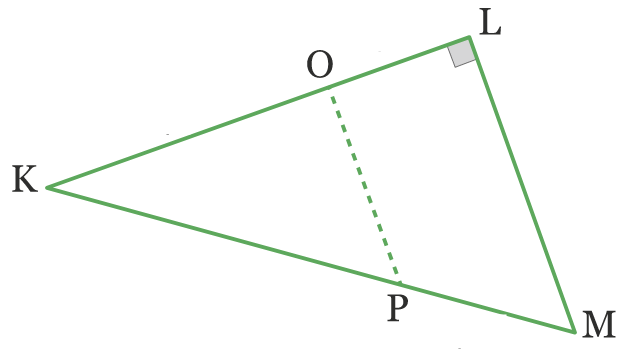
\includegraphics[scale=.3]{Exo2.png}\newline
Dans le triangle rectangle $LMK$, on a $KL = 9$, $LM= 12$, $KM=15$, $KO= 5,4$ et $MP= 6$. \begin{enumerate}
\item 
 Démontrer que les droites $(OP)$ et $(LM)$ sont parallèles.
 \item Quelle est la nature du triangle $KOP$ ? Justifier.
 \item 
 Calculer la longueur $OP$. 
\end{enumerate}

 
 \subsection*{Exercice 4}
 
 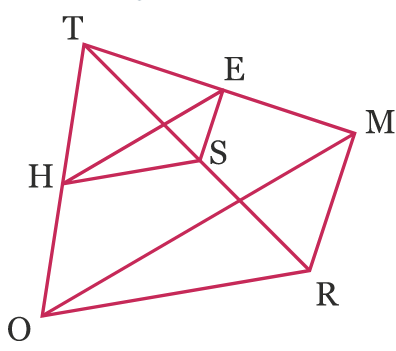
\includegraphics[scale=.4]{Exo4.png}\newline
 On suppose que $(HS)//(OR)$ et que $(ES)//(MR)$. 
 
 On donne $TH = 2$, $HO = 3$, $TS= 4$, et $TM= 9$. 
 
 \begin{enumerate}
 \item Calculer $TR$. 
 \item Calculer $TE$.  
 \item Démontrer que $(HE)//(OM)$. 
 \end{enumerate}
 

 	\end{document}
